\documentclass[12pt]{article}
\usepackage[utf8]{inputenc}
\usepackage{bm}                                     % bold in math env
\usepackage{import}                                 % import package
\usepackage{colortbl}
\usepackage[table]{xcolor}
\usepackage{url}
\usepackage{graphicx}
\usepackage{parskip}
\usepackage{fancyhdr}
\usepackage{vmargin}
\usepackage{geometry}
\usepackage{caption}
\usepackage{tcolorbox}                              % Beautiful box 
\usepackage{hyperref}
\usepackage{amsfonts,amsmath,amssymb,amsthm}        % all the math in one 
\usepackage{amsfonts}
\usepackage{tikz}                                   % drawing package
\usepackage[toc]{glossaries}                        % Module for glossary
\usepackage{xargs}                                  % more than one args in cmd
\usepackage{mathrsfs}                               % Cursive font
\usepackage{afterpage}                              % https://ctan.org/pkg/afterpage
\usepackage{float}                                  % Position of float
\usepackage[lofdepth=1,lotdepth]{subfig}
\usepackage{makecell}                               % \Xhline{NUM\arrayrulewidth}

% https://tex.stackexchange.com/questions/20575/attractive-boxed-equations
\usepackage{empheq}                         

\hypersetup{
    colorlinks=true,
    citecolor=magenta,
    linkcolor=black,
    filecolor=magenta,      
    urlcolor=cyan,
}
 

% { ..
% ..TODO REMOVE WHEN READY
\usepackage{lipsum}                                 
\usepackage[nottoc]{tocbibind}
\usepackage[firstpage]{draftwatermark}
\SetWatermarkText{DRAFT - ALPHA}
\SetWatermarkScale{3}
\SetWatermarkColor[rgb]{0.7,0.2,0.7}
% }

\setlength{\parindent}{0pt}     % Annule indentation automatique
\setlength{\parskip}{2ex}       % Saut de ligne

\title{Contrôle d'un agent via apprentissage par renforcement}
\author{Makdoud Nizam}
\date{\today}

% { -- Esthétique

\makeatletter
\let\thetitle\@title
\let\theauthor\@author
\let\thedate\@date
\makeatother

\pagestyle{fancy}
\fancyhf{}
\rhead{\theauthor}
\lhead{\thetitle}
\cfoot{\thepage}

% }


%% -- Redefinition
\renewcommand{\contentsname}{Table des matières} 
\renewcommand*\listfigurename{Liste des figures}
\renewcommand*{\acronymname}{Abréviations}
\renewcommand{\glossaryname}{Glossaire}

% https://tex.stackexchange.com/questions/5223/command-for-argmin-or-argmax
\DeclareMathOperator*{\argmin}{arg\,min} % thin space, limits underneath in displays

\makeglossaries
% -- simple test

\newglossaryentry{API}
{
    name=API,
    description={En anglais: \emph{Application program interface}, c'est un ensemble de protocoles, ou de contrats spécifiant le fonctionnant d'un programme. Dans le cas de ce rapport, cela correspond à un contrat entre l'application client et serveur (SE-STAR)}
}

\newglossaryentry{RL}
{
    name=RL,
    description={RL est l'acronyme de reinforcement learning qui en francais se traduit par apprentissage par renforcement.}
}


\newglossaryentry{GPU}
{
    name=GPU,
    description={En anglais: \emph{Graphics Processing Unit}, est un composant normalement utilisé dans la gestion des graphismes qui permet d'effectuer des calcules hautement parallèlisable de façon extrêmement rapide}
}

\newglossaryentry{PAAC}
{
    name=PAAC,
    description={Référence à une méthode en apprentissage par renforcement nommée \emph{Efficient Parallel Methods for Deep Reinforcement Learning }\cite{2017arXiv170504862C}. Elle se repose sur la même stratégie que l'A3C en utilisant une architecture synchrone permettant l'utilisation du GPU} 
}

\newglossaryentry{Wine}
{
    name=Wine,
    description={En anglais: \emph{Wine Is Not an Emulator}, est une application permettant l'utilisation d'application Windows sous Linux. Son nom vient du faite que de nombreuses personnes pensent a tort que Wine est un 'emulateur de Windows' or Wine a réimplémenté l'ensemble des appels systèmes dans le user space linux permettant à l'utilisateur de faire fonctionner une application Windows sous une distriubtion Linux}
}


\newacronym{gcd}{GCD}{Greatest Common Divisor}




% --------------------------------------------------------------------------
%%                                  BEGIN
% --------------------------------------------------------------------------

\begin{document}

\pagenumbering{roman}

% ============================================================
% Mise en page du titre
% cfhttps://www.overleaf.com/10351077tkgybggqnnsh#/38448375/
% ============================================================
\setmarginsrb{3 cm}{2.5 cm}{3 cm}{0 cm}{.5 cm}{1.5 cm}{0 cm}{0 cm} % Quick Hack 

\begin{titlepage}
	\centering
    \includegraphics[scale = 0.70]{./assets/ensem}\\[.75 cm]	% University Logo
    \textsc{\large École National Supérieur d'électricité et de Mécanique}\\[1.7 cm]	% University Name

	\rule{\linewidth}{0.5 mm} \\[.8 cm]
	{ \huge \bfseries \thetitle}\\[.65cm]
	\rule{\linewidth}{0.5 mm} \\[1.cm]
	
	\begin{minipage}{0.4\textwidth}
		\begin{flushleft} \large
			\emph{Auteur:}\\
			\theauthor
			\end{flushleft}
			\end{minipage}~
			\begin{minipage}{0.4\textwidth}
			\begin{flushright} \large
                \emph{Tuteurs:} \\
            Jerome Kodjabachian \\
			Marc Schoenauer \\
            Alexandre Kazmierowski
		\end{flushright}
	\end{minipage}\\[1.3 cm]
	
	\today\\[1. cm]

    \begin{minipage}[c]{0.45\linewidth}
        \hspace{-2cm}\includegraphics[width=1.4\linewidth]{./assets/thales}
    \end{minipage} \hfill
    \begin{minipage}[c]{0.45\linewidth}
        \includegraphics[width=1.4\linewidth]{./assets/inria}
    \end{minipage}

\end{titlepage}

\newpage

% =================================
% MACRO 
% =================================

\newcommand{\norm}[1]{\left\lVert\: #1 \:\right\rVert}
\newcommand\bsum{\mathlarger{\sum}}          % big summation
\newcommand\discountedReward{\sum_{k=0}^{\infty} \gamma^kR_{t+k+1}}
\newcommand\valueFunction{\mathbb{E_\pi}\bigg(\sum_{k=0}^{\infty} \gamma^kR_{t+k+1}  \:\bigg\vert\: s_t=s \bigg)}
\newcommand\QFunction{\mathbb{E_\pi}\bigg(\sum_{k=0}^{\infty} \gamma^kR_{t+k+1}  \:\bigg\vert\: s_t=s, a_t=a \bigg)}

% Policy with color to highlight the conditional probability (policy color -> policyc)
\newcommand{\policyc}[1]{
    \textcolor{#1}{
        \underbrace{\pi(x\:,\:a)}_{p\:(a \:\vert\: s)}
    }
}

\newcommand{\dynamicsc}[1]{
    \textcolor{#1}{
        \overbrace{T(s',r , s, a)}^{p(s',r \vert s, a)}
    }
}


% =================================
% Résumé - Remerciement
% =================================


% Just the default setting 
\setmarginsrb{3 cm}{2.5 cm}{3 cm}{2.5 cm}{1 cm}{1.5 cm}{1 cm}{1.5 cm}
\thispagestyle{empty}

\section*{Remerciements}
\bigskip
Je tiens à remercier chaleureusement toutes les personnes qui m'ont accompagnées durant ce stage pour faire de ces six mois une expérience  profitable sur le plan professionnel et agréable sur le plan personnel.


\noindent Tout d'abord, je remercie Jérome Kodjabachian, Marc Shoenauer et Christophe Meyer pour m'avoir donné l'opportunité d'effectuer ce stage, de m'avoir conseillé et  permis de m'épanouir durant ces six mois.


\noindent Je remercie également Alexandre kazmierowski pour son soutien, ses conseils assidus et sa disponibilité sans laquelle je n'aurais pas pu avancer sur certains points de ce stage.   


\noindent Enfin, je tiens à remercier l'ensemble de l'équipe AS&BSIM, pour sa sympathie et sa disponibilité.
\newpage
\thispagestyle{empty}
\section*{Abstract}
\bigskip

Artificial intelligence is a growing field which aims to improve task automation. Through this internship, a subfield of artificial intelligence named reinforcement learning has been explored.

Reinforcement learning deals with issues governed by a set of rewards. For example, the classical problem in reinforcement learning is the control of agent through one place to another. The agent receives a reward when it arrives to the final place.  The goal of our control is to find the optimal sequence of actions that maximises the cumulated rewards, which is, for our example, to reach to goal within the shortest time.

THALES is involved in the infrastructure security design, and aims to ensure the security of infrastructures by created plans to scenarios generated by SE-STAR. 
SE-STAR is a simulation capable of created multiple scenarios which may involve a large number of agents. SE-STAR uses internal drives (like hunger, fear, stress ...) to control the mass of agents but these internal drives has to be carefully design to accomplish a scenario (like a fight in a gare).

We choose another way to control agents that uses only rewards to automatically find the optimal behaviour that correspond to a given scenario.
Notably, we have worked on the control of an agent in a simulated environnement created by the THALES' internal biomimetic simulation SE-STAR.

We will propose various architectures and reinforcement learning algorithms to allow an agent to move in its simulated environnement by its own internal motivations to find our specified goal. The novelty of this approch is to find a policy with a weakly informative input like the partial vision of the agent which banned the use of other traditionnal control algorithms. 

Non-exhaustively, the internship has been divided in five periods:

\begin{itemize}
    \item Bibliographic and litterature search.
    \item Application of main algorithms on simple environnements.
    \item Development of reinforcement learning algorithms on 2D and 3D environnements used by researchers to benchmark their controllers. 
    \item Design of a wrapper around the simulation SE-STAR to support the use of our external algorithm.
    \item Research of algorithms based on intrinsic motivations (or curiosity) to help the agent to find the optimal policy in difficult 3D environnements like those created by SE-STAR. 
\end{itemize} 

\newpage


\section*{Résumé}
\bigskip

L'apprentissage automatique est un domaine subissant actuellement une forte expansion, permettant une automatisation de nombreuses tâches. A travers ce stage, nous avons exploré une sous partie de l'apprentissage automatique qui se nomme l'apprentissage par renforcement profond. 

Ce domaine vise à résoudre des problèmes qui sont régis par des récompenses. Par exemple, nous pouvons imaginer le problème d'un agent ayant pour but d'aller d'un point A à un point B, une récompense serait donnée à l'agent dès qu'il attendra le point B. Notre objectif serait de trouver la politique optimale de l'agent pour maximiser la quantité de récompenses reçues. Dans notre exemple, l'agent aurait à apprendre la séquence d'actions qui permettrait d'aller jusqu'au point B, et ainsi d'obtenir le maximum de récompenses. En particulier, nous travaillerons à l'aide d'un logiciel de simulation bio-inspiré qui se nomme SE-STAR. 

THALES est impliqué dans la conception d'infrastructures critiques. THALES a pour objectif de garantir la sécurité des infrastructures. Pour cela, elle utilise le logiciel SE-STAR qui est une simulation ayant pour but de créer des plans répondant à des scénarios possibles dans l'infrastructure concernée. SE-STAR a la capacité de gérer un grand nombre d'agents simultanément. Pour contrôler ces individus, SE-STAR utilise des motivations (faim, stress, peur ...), néanmoins, pour contrôler une masse d'individus, il faut être précis dans la conception de ces motivations pour accomplir un scénario.

Nous avons choisi une autre voie pour contrôler les agents qui n'utilise que la spécification des récompenses pour générer un comportement correspondant à celui souhaité pour un scénario.
Nous avons donc travaillé sur le contrôle d'un agent dans une simulation crée par SE-STAR.

Nous proposerons une architecture et des algorithmes d'apprentissage par renforcement permettant à un agent de se déplacer dans l'environnement simulé à la recherche de la sortie de façon non supervisée (ou faiblement supervisée). L'intérêt de notre approche est qu'elle utilise des entrées extremment bruitées et partielles (la vision de l'agent) ce qui empêche toutes stratégies de contrôles usuellement appliquées.

De manière non exhaustive, nous pouvons définir ce stage en cinq périodes: 
\begin{itemize}
    \item Découverte et recherche bibliographique.
    \item Application des principaux algorithmes sur des cas simples.
    \item Élaboration d'algorithmes de renforcements profonds sur des environnements 2D et 3D utilisés par les chercheurs pour comparer la performance de leurs méthodes
    \item Conception d'un outil autour de SE-STAR pour supporter les algorithmes d'apprentissage par renforcement.
    \item Recherche autour d'une solution adaptée spécifiquement à l'apprentissage par renforcement profond dans le cadre problématique des environnements labyrinthiques.
\end{itemize}

Ci dessous une représentation des grandes périodes pendant ce stage:

\begin{center}
\includegraphics[scale=.5]{./assets/globale.png}
\end{center}

\newpage

% =================================
% Table des matières et autres
% =================================

\thispagestyle{empty}
\listoffigures   \newpage

\thispagestyle{empty}
\tableofcontents \newpage


% =================================
% Corps du rapport
% =================================

\hypersetup{linkcolor=teal}

\pagenumbering{arabic}
\setcounter{page}{1}

\section{Introduction}

Dans le cadre de ma formation d'ingénieur à l'\emph{École Nationale Supérieure d'électricité et de Mécanique}, j'ai réalisé un stage du 2 février 2017 au 2 août 2017 au sein du laboratoire ThereSIS de THALES Services à Palaiseau, dans le campus de Saclay. J'ai eu l'occasion pendant ce stage d'effectuer de nombreux séjours à l'INRIA Tao pendant lesquels j'ai pu m'entretenir avec des chercheurs en apprentissage par renforcement et me tenir au courant des avancées dans le domaine de l'intelligence artificielle.

J'ai réalisé ce stage au sein de l'équipe AS&BSIM (Adaptative Systems and
Biomimetic Simulation), qui travaille principalement sur le logiciel \textbf{SE-STAR}. Il s’agit d’un environnement synthétique où évoluent de nombreux agents virtuels, chacun disposant d’un modèle cognitif. 

Dans le cadre de ces simulations, je me suis intéressé à la navigation d'un agent en utilisant l'apprentissage par renforcement profond pour contrôler l'agent dans son environnement. En particulier, la contrainte imposée sur le contrôle de l'agent est qu'en entrée du contrôleur, nous n'avions accès qu'à une image 2D d'un environnement 3D (en l'occurrence SE-STAR).



\subsection{Contexte du stage et de l'entreprise}

Le groupe THALES est une multinationale française employant 67 000 salariés
dans 56 pays. Si l’entreprise est connue auprès du grand public pour sa présence
sur le marché de la défense, elle opère aussi sur plusieurs marchés duaux (à la
fois civils et militaires) : l’aéronautique, l’espace et la sécurité, ainsi que sur le
marché civil du transport terrestre. Les problématiques de traitement et
interprétation des données ainsi que d’aide à la prise de décision sont au cœur
de l’activité du groupe. Afin de renforcer la position du groupe dans l’innovation
autour des nouvelles technologies, les activités de recherche et développement
sont au cœur de l’entreprise, représentant 20\% de ses revenus. THALES possède
un réseau international de laboratoires qui coopèrent avec des universités et des
laboratoires de recherche publics.

THALES Services est une division de THALES, dont l’activité se situe autour des
systèmes d’information et de communications sécurisés.
ThereSIS (THALES European Research for E-Government & Secured Information
Systems) est le laboratoire de recherche en systèmes d’information de THALES
Services. Il est situé sur le site de THALES Research and Technology à Palaiseau.
Les équipes en place ont pour mission de tester des technologies
innovantes, afin de déterminer si elles peuvent être exploitées au profit du
groupe THALES et de ses clients. Des démonstrateurs sont mis en place pour
présenter aux clients des cas concrets d’utilisation de ces technologies
novatrices, parmi lesquelles on peut trouver le cloud computing, les systèmes de
vidéosurveillances, les simulateurs.

Depuis quelques années, ThereSIS a mis l'accent sur les technologies autour de l'intelligence artificielle, et propose une expertise dans ce domaine. Cela permet à THALES d'être un acteur de poids dans les domaines de de la cybersécurité et de la sécurité des infrastructures critiques (gares, aéroports, ...).

ThereSIS propose des projets de recherche ou répond à des appels d’offres
émanant d’entreprises ou de groupes finançant la recherche industrielle. L’intérêt
des clients pour les prototypes présentés peut mener à une phase
d’industrialisation et de commercialisation prise en charge par les départements
de production de THALES Services.

\bigskip
En quelques chiffres, voici une vue de la taille de THALES et de l'importance donnée à la R&D: 
\bigskip
\begin{figure}[!h]
\centering
\includegraphics[width=.9\linewidth]{./assets/thales_chiffres}
\caption{THALES en quelques chiffres}
\medskip
\small
\end{figure}
 
\subsection{Description du sujet de stage}
\subsubsection{L'environnement de simulation: SE-STAR}

SE-STAR est un logiciel de simulation dans des environnements modélisés à partir
de lieux réels. Dans l’environnement virtuel interagissent en temps réel des
agents représentant des personnes. Il est conçu en particulier pour les
infrastructures critiques (stations de métro, gares, aéroports).
Il peut gérer en temps réel un grand nombre d’agents (plus de 10 000), permettant de nombreuses interactions avec l’environnement qui peut être facilement modifié par l’utilisateur (ajout d’objets tels que des caméras de surveillance, des distributeurs de boissons, des bancs, etc.). La simulation cherche à représenter de manière réaliste le comportement des usagers de ces infrastructures. 

Dans le contexte de ce stage, nous allons restreindre SE-STAR à la modélisation d'un environnement simple contenant un seul agent. 

\midskip
\begin{figure}[ht!]
    \subfloat[Environnement pour contrôle]{\includegraphics[width = .43\linewidth]{./assets/SESTAR/envsestarcolor.png}}\: 
    \subfloat[Simulation d'une gare]{\includegraphics[width = .5\linewidth]{./assets/SESTAR/sestarmetro.png}}
    \caption{Exemple d'utilisation de SE-STAR}
\label{some example}
\end{figure}

\subsubsection{Objectif du stage et contraintes identifiées}


L'objectif de ce stage est de proposer un contrôle d'un agent de l'entrée de l'environnement à la sortie de l'environnement en évitant des zones considérées comme dangereuses. Néanmoins, nous possédons des contraintes sur notre contrôle:     

\begin{enumerate}
    \item \textbf{L'environnement est inconnu de l'agent:}
    \smallskip
    
    La première contrainte de notre objectif est que notre environnement est inconnu. En effet nous souhaitons développer un algorithme de contrôle que soit capable de proposer un asservissement fiable pour tout environnement proposé par SE-STAR. L'impératif de généralisation est une contrainte forte pesant sur le choix technologique pour réaliser ce contrôle. En effet, un asservissement classique repose sur la connaissance de la dynamique du système qui n'est pas disponible dans notre cas et , pire encore, est fluctuante en fonction des environnements.
    
    \item \textbf{Le contrôle doit être robuste aux changements d'environnements:}
    \smallskip
    
    Pour être utile, il faut que notre agent apprenne à se mouvoir d'un point A à un point B. De plus, notre algorithme d'apprentissage ne doit pas se suffire à apprendre par coeur la séquence d'actions pour rejoindre la sortie mais doit apprendre à se repérer et voir les points d'intérêts permettant de trouver la sortie quelque soit l'environnement. Nous recherchons une approche analogue à la façon humaine  pour sortir d'un environnement (longer les murs, chercher des indices visuels indiquant la sortie ...).
 
    \item \textbf{Les entrées de la commande sont données par la vision de l'agent:}
    \smallskip
    
    Une des difficultés qui empêche l'utilisation des outils de la théorie du contrôle, vient du format des entrées. Nous devons bâtir un algorithme de contrôle se basant sur des images partielles d'un environnement. Comme un humain lâché dans un labyrinthe, il n'aura pas accès à une image complète du labyrinthe mais uniquement une vue partielle possiblement bruitée. Notre agent devra, à partir d'une information incomplète, réussir à déterminer une séquence d'actions lui permettant de trouver la sortie.
    
  
\end{enumerate}

\subsubsection{Défis et choix technologiques}

Nous cherchons un algorithme de contrôle assez générique pour ne nécessiter en entrée que des images (tableaux de pixels). Un des défi de ce stage est de permettre à  l'agent d'être capable de trouver les repères les plus adaptés pour réussir sa mission quelque soit l'environnement.

Cela implique que nous ne recherchons pas seulement une solution adaptée à un environnement particulier. Nous souhaitons un agent capable de généraliser à un ensemble d'environnements similaires. 

Les nombreuses contraintes et les défis technologiques impliquent une décomposition de l'algorithme choisi en deux grandes étapes:

\begin{enumerate}
    \item L'agent explore l'environnement et apprend simultanément une politique optimale pour arriver à la sortie.
    \item Nous nous assurons que l'agent est capable de trouver une bonne politique sur des environnements similaires pour vérifier que l'agent n'a pas juste \emph{appris par coeur une solution}\footnote{Nous reviendrons plus tard sur la signification de la généralisation qui est un problème central}.
\end{enumerate}

Se pose naturellement la question du choix de la technologie pour réaliser cet apprentissage.
La contrainte de généralisation nous pousse à utiliser l'apprentissage profond (ou \emph{deep learning}). L'apprentissage profond a prouvé son efficacité dans sa capacité à être pertinent à un grand nombre d'entrées possibles.  
La distinction entre généralisation et apprentissage par coeur des données est particulièrement importante dans ce domaine. Les méthodes qui en sont issues ont prouvé leurs capacités à trouver des solutions à des problèmes nouveaux (jamais utilisés en entrainement).

Il nous faut un domaine s'attaquant à des environnements compliqués, observés de manières partielles, et possiblement changeant au cours du temps. L'apprentissage par renforcement propose une manière d'aborder ces d'environnements complexes. 

Ainsi, nous avons proposé une méthode alliant l'apprentissage profond pour gérer les entrées du système avec l'apprentissage par renforcement pour réaliser un agent capable de naviguer dans un environnement pour y découvrir une sortie en ayant comme donnée unique sa vision.

\input{corps/preliminaire/architecturefonctionnementrl.tex}
\input{corps/preliminaire/TDA3CDeepQLearning.tex}
\subsubsection{Platformes utilisables pour garantir le fonctionnement de nos algorithmes}
\label{sssec:benchmark}
Malgré que nos algorithmes aient pour but d'être déployés sur l'environnement interne de Thales SE-STAR, il nous a fallut trouver des environnements suffisamment complexes pour tester la robustesse de nos agents mais aussi suffisamment simples pour ne pas devoir attendre un temps infiniment long pour avoir notre réponse. De plus, la connection de nos algorithmes avec SE-STAR est un enjeu essentiel et a apporté son lot de difficulté. Il n'était donc pas raisonnable d'attendre ni de tester nos agents sur cette plateforme.

Il existe de nombreuses plateformes dédiées à l'apprentissage par renforcement. Nous avons choisi de nous concentrer sur des environnements proches de SE-STAR. Ainsi, de nombreuses études en \gls{RL} utilisent des jeux Atari en 2D et 3D. Nous allons donc nous baser en partie sur ce type d'environnement.

Vous pouvez voir page suivante plusieurs types d'environnements sur des plateformes différentes:

\begin{enumerate}
    \item \textbf{Gym\cite{1606.01540} - OpenAI}\\
        Gym est une plateforme qui met à disposition des jeux Atari et des simulations typiques en contrôle (Cartpole, MountainCar ...). La plateforme fournie une \gls{API} permettant de réutiliser nos codes sur l'ensemble des simulations qui sont fournis par Gym.
    
        L'\gls{API} de Gym étant simple, nous avons décider de nous baser sur cette API pour la construction d'un wrapper\footnote{cela consiste en un logiciel intermédiaire qui a pour but de faire le lien entre deux codes.} autour de la simulation interne de Thales SE-STAR.
    
    \item \textbf{Universe - OpenAI}\\
    Universe est une autre plateforme mettant à disposition une multitude de jeux très différents les uns des autres (2D, 3D, textes ...). Certains sont récents et demandent une certaines réflexions (Portal, age of empire, ...). L'organisation de Universe est plus complexe que celle de Gym et impose la prise en compte de plus d'éléments (réseau, possible lag, infrastructure ...). 
    
    Universe propose donc des environnements plus difficiles à tout point de vue que Gym néanmois cette plateforme n'est pas encore utilisé par les chercheurs et on peut douter de la maintenance du projet Universe (OpenAI semble mettre en avant Gym\footnote{Le projet n'a pas été mis à jour depuis 8 mois sur le githubdu projet.})
    
    \item \textbf{DeepmindLab\cite{DBLP:journals/corr/BeattieLTWWKLGV16} - Deepmind / Google }\\
        Le deepmindlab est une seul simulation de labyrinthe 3D très proche de notre application. Le problème est la difficulté d'utilisation de cette plateforme. Ainsi, nous n'avons pas utilisé cette ressource néanmoins elle est pertinante et est une cible pour tester nos algorithmes.
    
    \item \textbf{Doom - Vizdoom\cite{DBLP:journals/corr/KempkaWRTJ16}  }\\
        Doom est un jeu PC de tir à la première personne. Cet environnement est devenu un classique dans la communauté \gls{RL} pour tester les algorithmes d'apprentissage par renforcement. A tel point que l'université de Poznan à créer une compétition d'\gls{IA} basée sur Doom. L'intérêt de cet environnement, contrairement au précédant, est qu'il est plus complet avec un ensemble d'actions possibles conséquent. De plus, l'environnement de Doom met en lumière des difficultés pour les \gls{IA} en matière d'exploration de l'environnement et est donc un terrain de jeu pour résoudre ou proposer des algorithmes résolvant ce type de problème.
    

\end{enumerate}

\bigskip
\begin{figure}
\centering
\includegraphics[width=.9\linewidth]{./assets/GYM/gym2}
\caption{Exemple d'environnements GYM (Open AI)}

\bigskip

\includegraphics[width=.9\linewidth]{./assets/GYM/gym}
\caption{Exemple d'environnements Universe (Open AI)}

\bigskip

\includegraphics[width=.6\linewidth]{./assets/GYM/deepmindlab}
\caption{Exemple d'environnements DeepmindLab (Deepmind (Google)) }
\medskip
\small
\end{figure}



\input{corps/preliminaire/deeplearning.tex}                    \newpage
\definecolor{Gray}{gray}{0.85}
\definecolor{LightCyan}{rgb}{0.88,1,1}

\section{Interface entre SE-STAR et le contrôleur}

Une grande partie de ce stage a tourné autour de l'interaction des algorithmes d'apprentissage par renforcement et SE-STAR (cf \ref{globalViewProject}). Cette partie sera consacrée à l'explication de l'architecture mise en place autour de SE-STAR pour la connection du contrôleur et de SE-STAR.
L'architecture proposée est composée de la création d'une \gls{API} simple pour communiquer avec SE-STAR et d'une interface bas niveau pour intégrer l'\gls{API} haut niveau (réalisée par Alexandre  kazmierowski).

Nous discuterons des diverses difficultés que nous avons rencontrées, des limites de notre architecture et des améliorations possibles.


SE-STAR est à la base un logiciel de simulation interne à THALES. SE-STAR a été prévu pour permettre une communication via son \gls{API} réseau. Pourtant, l'API n'a pas été pensé pour un pilotae d'un agent par renforcement .Le contrôle des agents dans SE-STAR se base sur des stimulis internes motivationnels qui peuvent être configurés en fonction du rôle que l'on souhaite donner à un agent. Nous ne rentrerons pas dans les détails du fonctionnement original qui est complexe et orthogonal à notre objectif. Notre but est justement de créer un contrôle automatique se basant sur des stimulis extrinsèques (donnés par l'environnement) reposant sur la théorie de l'apprentissage par renforcement profond.

SE-STAR est un logiciel complexe. Il a donc fallu créer une interface étant la moins intrusive possible sur le code source de SE-STAR. L'objectif était de produire un code réutilisable quelque soit l'environnement. Nous nous rendrons compte que ce choix implique une perte en performance.

\begin{figure}[!h]
\centering
\includegraphics[width=.9\linewidth]{./assets/interfaceReseau/overviewInterface}
\caption{Vue globale de l'interaction entre le contrôleur et SE-STAR}
\end{figure}

\subsection{Analyse fonctionnelle de l'\gls{API} choisie}

Nous allons profiter de la simplicité de notre API pour l'expliquer. En apprentissage par renforcement,  un agent reçoit l'état dans lequel il se trouve. A partir de celui-ci, il interagit avec l'environnement qui lui répond en envoyant le prochain état et la récompense associée à l'état. Nous allons nous baser sur ce fonctionnement pour créer notre \gls{API}. 


\bigskip

% { --

\setlength{\arrayrulewidth}{.7mm}
\setlength{\tabcolsep}{12pt}
\renewcommand{\arraystretch}{2.}

\begin{center}
{\rowcolors{2}{white!80!gray!50}{gray!50!white!60}
\begin{tabular}{ |p{2cm}|p{8cm}|  }
\hline
\multicolumn{2}{|c|}{\gls{API} Client} \\
\hline
Fonction & Explication \\
\hline
Reset & Reset a pour but de redémarrer la simulation (obligatoire en cas de fin de partie ou si un certain temps est dépassé) \\
\hline
Step & \begin{enumerate}
\item Entrée: l'action effectuée
\item Sortie: une liste contenant l'état suivant, la récompense reçue, un booléen indiquant si la simulation est terminée et un dictionnaire donnant une multitude d'informations sur la simulation.
\end{enumerate} \\
\hline
Connect & Une fonction nous permettant d'établir une connection à distance avec un Windows distant. Nous ne parlerons pas de la méthode de connection à distance qui est assez complexe et reposant sur des outils tiers (Winexe, ...) \\
\hline
\end{tabular}
}
\end{center}

% -- May need change if set.. are not local }


L'\gls{API} est simple mais correspond exactement à la boucle classique en renforcement. Alexandre Kazmierowski a construit le serveur répondant à ces appels. L'outil créé par M. Kazmierowski permet l'interconnexion entre SE-STAR et le client (le contrôleur).

\subsection{Principales limites et contraintes}

La simulation SE-STAR fonctionne actuellement uniquement sur Windows. Cela pose un problème car les différents outils, pour créer des algorithmes de Deep Learning, utilisent une distribution linux\footnote{Notamment les frameworks de deep learning sont exclusivements sous linux (Tensorflow, Pytorch, Caffe ...)}. Les échanges réseaux entre Linux et Windows limitent drastiquement le nombre d'images par seconde que peut recevoir l'agent (définissant donc la vitesse de simulation) car l'envoi d'un tableau de pixels sur le réseau est intrinsèquement coûteux. 

De plus, nous avons été confronté à de nombreux problèmes de déconnections impromptus qui ont nécessités la mise en place de mécanismes de reconnections automatiques. Néanmoins l'architecture mise en place manque encore de stabilité et n'est pas robuste à tous les types d'erreurs pouvant être rencontrés.

L'algorithme utilisé pour contrôler l'agent dans SE-STAR a été l'\gls{A3C}\footnote{on parlera pour la version la plus simple du contrôleur.} qui repose sur de multiples agents qui jouent dans l'environnement de façon asynchrone. Cela multiplie le nombre d'appels réseau et joue sur la stabilité de celui-ci, cela accroît la latence des appels agent (SE-STAR) / algorithme (Contrôle). De façon empirique, nous nous apercevons qu'il y a des problèmes dès que le nombre d'agents est supérieur à six. Cela s'explique en partie par le fait que SE-STAR est un logiciel demandant beaucoup de ressources, Or celui-ci n'a jamais été prévu pour une utilisation demandant de faibles ressources\footnote{SE-STAR est prévu pour contrôler plusieurs milliers d'agents or dans notre cas d'usage nous souhaitons en contrôler qu'un seul.}. Ainsi la multiplication des instances de SE-STAR peut causer des problèmes sur la machine coté serveur si elle n'a pas assez de puissance. Alexandre  Kazmierowski nous a permis d'alléger les ressources demandées, permettant d'augmenter le nombre d'agents.

Nous pouvons dès lors nous demander si la stratégie asynchrone d'entraînement est viable.
Une problématique inhérente aux algorithmes de renforcement, qui découle de l'utilisation du deep learning, est le besoin de décorréler les états lors de l'entraînement . Or dans le cadre de nos algorithmes, cela s'avère difficile. La stratégie d'entraînement asynchrone permet la décorrélation des états lors de l'apprentissage.


En ajoutant les défaults de l'A3C, nous pouvons nous demander si d'autres algorithmes ne seraient pas plus pertinents\footnote{Il y a quelques semaines dans la communauté \gls{RL}, il y a eu une profonde remise en question de l'utilité de l'approche asynchrone, nous parlerons plus tard de la PAAC comme architecture synchrone potentiellement utilisable.}.

\subsection{Compromis et solutions envisagées}

Dans cette partie, nous allons expliquer les solutions envisagées pour éviter de surcharger le réseau. Avant cela, il convient de revenir sur certaines contraintes sur le contrôle. En particulier, nous souhaitions avoir un contrôle qui est le moins intrusif possible sur l'environnement en l'occurrence SE-STAR.

Nous allons cependant proposer une méthode qui reste intrusive mais permet de résoudre en partie les problèmes liés à la multiplication des instances de SE-STAR et de réduire les appels réseau . 

La méthode qui sera développée se nomme PAAC: Efficient Parallel Methods for Deep Reinforcement Learning \cite{2017arXiv170504862C}. Nous ne rentrerons pas dans les détails de l'algorithme car il est similaire à l'\gls{A3C} \cite{DBLP:journals/corr/MnihBMGLHSK16}. Néanmoins,il propose une approche synchrone permettant l'utilisation du GPU. L'idée de ce papier est de proposer une architecture synchrone permettant de décorréler les états utilisés pour l'entrainement. A chaque pas, le contrôleur va décider quelles actions vont effectuer un ensemble d'agents. Le contrôleur va récupérer l'ensemble des états et des récompenses pour l'apprentissage et le choix de la nouvelle action. Quand le contrôleur rentre en phase d'apprentissage, il a un ensemble de transitions (état précédant, état actuel, action, récompense) décorrélées (car venant d'agents différents). Les premiers essais sont encourageants mais l'apprentissage n'est pas assez stable.

\begin{figure}[h!]
\begin{center}
\includegraphics[scale=.4]{./assets/interfaceReseau/paaca3c}
\caption{Comparatif des algorithmes PAAC / A3C en mettant l'accent sur les problématiques réseaux}
\end{center}
\end{figure}

Nous remarquons que les principaux problèmes qui découlent de la stratégie asynchrone d'entrainement (A3C) sont liés à la communication réseau mais pas seulement. Un stratégie asynchrone exclue l'utilisation du \gls{GPU}. La stratégie synchrone de la \gls{PAAC} permet l'utilisation du GPU mais impose que la simulation soit capable de gérér un ensemble d'actions en entrées. De plus, la question des transferts sur le réseau n'est pas résolue par cette approche. 

La véritable question est de savoir s'il n'existe pas d'autres approches qui suppriment la nécessité du réseau ou qui reposent sur des outils spécialement crées pour gérer les difficultés inhérentes aux réseaux. Nous verrons rapidement deux approches idéales se basant sur un outil Docker \cite{Merkel:2014:DLL:2600239.2600241} et sur l'utilisation de \gls{Wine} (qui permet de faire fonctionner des applications Windows sur Linux)

\subsection{Solutions idéales}

\subsubsection{SE-STAR sous linux via \gls{Wine}}
Notre objectif a été d'utiliser SE-STAR nativement sous Linux. Pour cela, il y a deux solutions. 
Premièrement, nous pouvons compiler directement SE-STAR pour Linux. Le problème est que le logiciel a été pensé pour une utilisation Windows et utilise certaines librairies uniquement disponibles sur Windows. Nous ne savons pas si cela est possible même si cela aura le mérite d'être essayée. 
Deuxièmement, nous pouvons passer sous Wine pour utiliser une application Windows. Après une phase de configuration compliquée pour utiliser Wine, nous avons été en capacité d'utiliser SE-STAR sous Linux et d'utiliser l'\gls{A3C}. Nous avons remarqué des interruptions complètes de SE-STAR au bout d'une dizaine de minutes. Pour l'instant, il est difficile de savoir ce qui est responsable de ces interruptions. Nous pensons toujours que Wine est une solution viable. Il est reste néanmoins à comprendre l'origine des problèmes. Une des problématiques qui survient avec l'utilsation de Wine est que les fonctionnalités permises par SE-STAR ne sont pas entièrement prise en charge par Wine. Cela nous oblige donc à passer par une version obsolète de Wine et possiblement moins stable.

\subsubsection{Une architecture scalable d'entrainement via Docker}
Nous allons présupposer que nous avons un moyen d'utiliser SE-STAR sous Linux. Nous exploiterons Docker (qui est un système de conteneurisation, qui groupe une application avec un environnement Linux léger configuré au préalable). Cela permet, en spécifiant les dépendances de SE-STAR, de pouvoir déployer dans un réseau n instances de SE-STAR et de simplement utilser le \emph{swarm mode} de docker pour avoir une gestion du réseau (load balancing, ...). Nous  pourrions imaginer déployer dans un cluster de cpu (ou gpu) plus de 1000 instances de SE-STAR gérées par le swarm mode de Docker. Ce genre d'architecture a déjà été utilisée.Cela pourra être mis en place dès que SE-STAR sera disponible sous Linux.

\begin{center}
\includegraphics[scale=.65]{./assets/interfaceReseau/docker}
\captionof{figure}{Simple vue d'ensemble de l'utilisation de Docker en swarm mode}
\end{center}


Le swarm mode de Docker est une architecture composée d'un (ou plusieurs) noeud manageur qui a pour but de contrôler les noeuds enfants, de gérer le load balancing, la gestion des erreurs des noeuds enfants ... En ayant des conteneurs avec les dépendances requises par SE-STAR et l'application SE-STAR dans chaque conteneurs enfants, cela permet d'utiliser les algorithmes classiques d'apprentissage par renforcement profond à un échelle industrielle.

\subsection{Conclusion sur les questions d'interfaces et de réseaux}

A travers ce chapitre, j'ai essayé de vous expliquer les principaux enjeux dans le cadre de l'interface entre SE-STAR et les algorithmes d'apprentissage. Sur des cas jouets, ces problématiques ne font pas surfaces néanmoins, dans des applications industrielles nous sommes obligés de réfléchir à l'architecture dans laquelle nous allons déployer nos algorithmes et nos applications. Or, les \gls{frameworks} d'apprentissage et les applications peuvent être destinées à des environnements différents ou pire avoir des dépendances contradictoires. Il est donc essentiel  d'utiliser des applications capables d'isoler une application afin que celle-ci puisse être  disponible sur le réseau dans le but de pouvoir permettre la communication entre les applications.

Ci-dessous, un schéma récapitulatif de l'architecture idéal (qui a été partiellement mise en place durant le stage).


\begin{center}
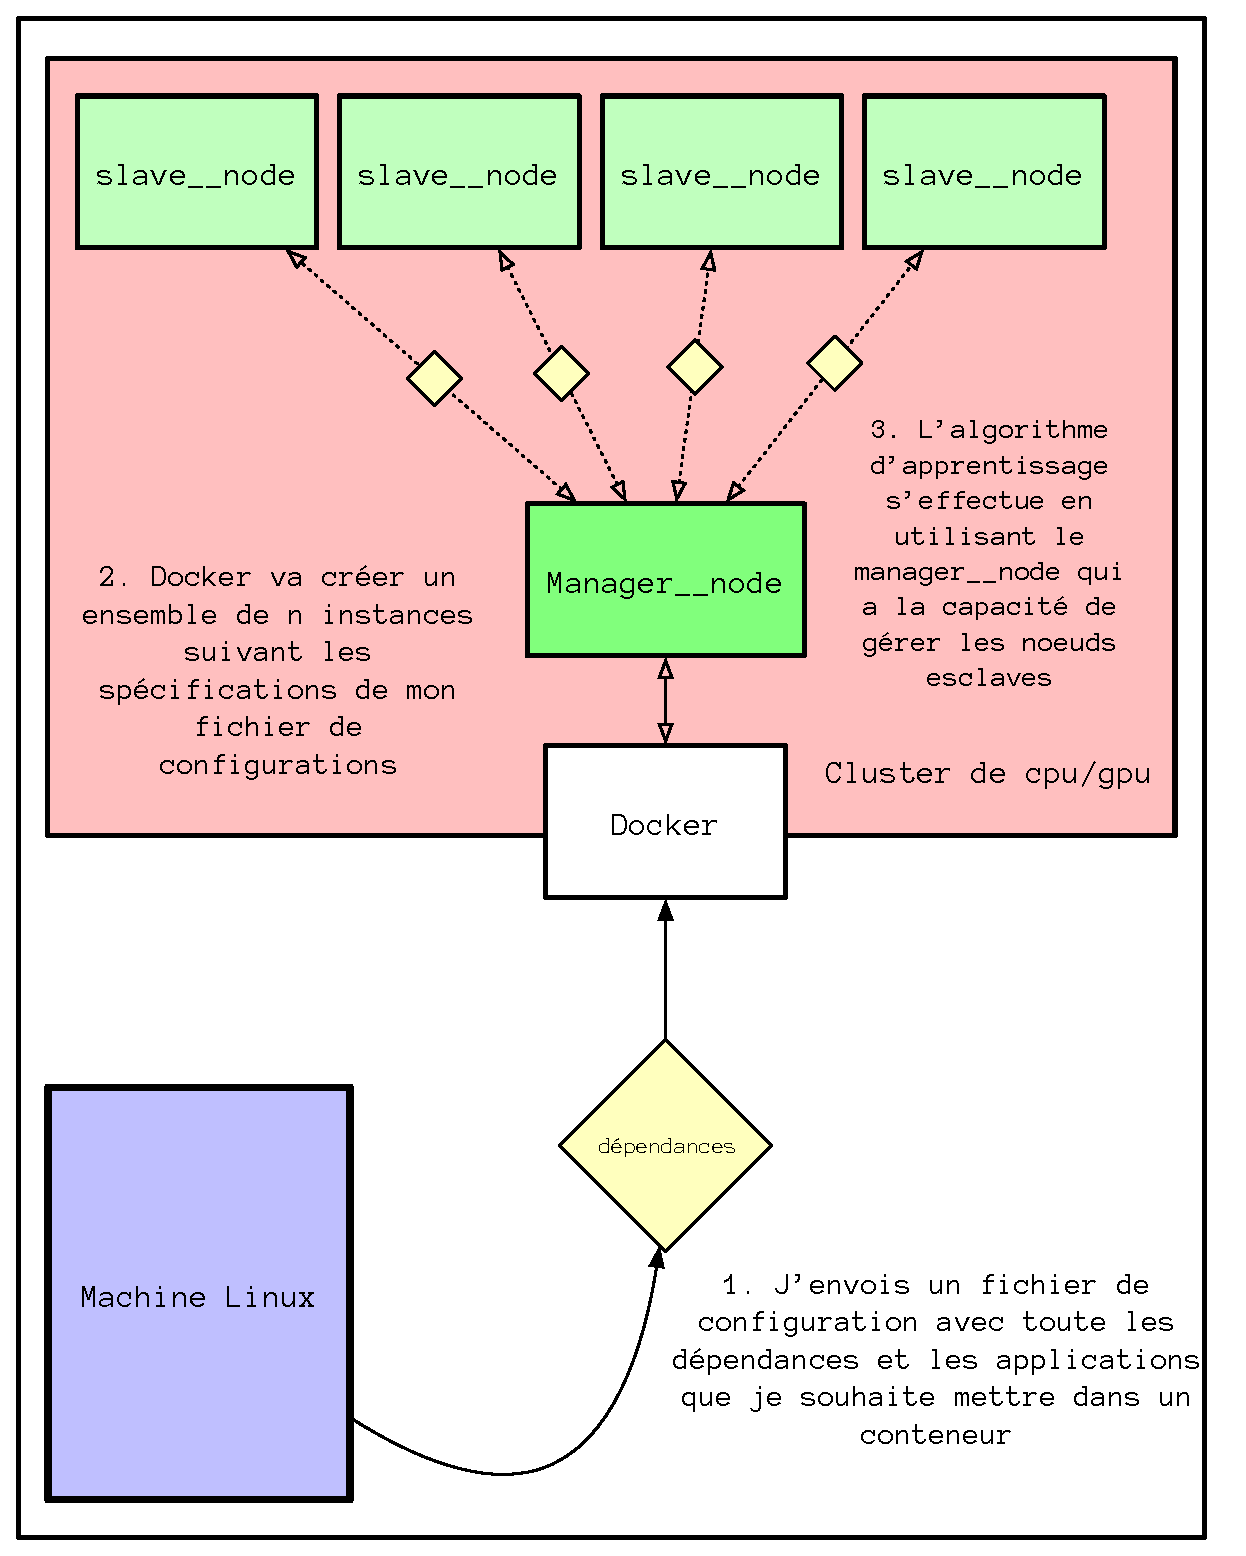
\includegraphics[scale=.7]{./assets/interfaceReseau/interfaceResume.eps}
\captionof{figure}{Vue d'ensemble de l'architecture partiellement mise en place dans le cadre de l'apprentissage de l'algorithme}
\end{center}
               \newpage
\section{Contrôle d'un agent via la simulation SE-STAR par renforcement profond}

Cette partie sera consacrée au fonctionnement du contrôle appliqué à SE-STAR. Dans le but de comprendre les choix entrepris, nous commencerons par expliquer comment fonctionne l'algorithme d'apprentissage par renforcement utilisé pour SE-STAR. Puis, nous expliquerons les faiblesses de cet algorithme (dans le contexte de SE-STAR). Enfin, nous introduirons un module de curiosité qui a pour but d'améliorer l'apprentissage et donc le contrôle de l'agent.


Nous considérons SE-STAR comme un environnement sans faire mention des problématiques liées à l'interface contrôleur / SE-STAR, ou des problématiques liés aux réseaux qui ont été développé dans la partie précédente. 

\subsection{Le choix d'un algorithme efficace pour le contrôle d'un agent dans SE-STAR.}

Il existe dans la littérature un panel très large d'algorithmes qui sont potentiellement puissants. Or, pour des questions de temps, nous n'avons pas été capable d'essayer tous les algorithmes. Nous avons donc dû faire un choix. 

Nous allons à travers cette partie, donner les principales raisons qui nous ont poussées à nous diriger vers un apprentissage par renforcement profond. 

Tout d'abord, les spécificités de SE-STAR impliquent le non-usage des algorithmes \emph{model based} (basés sur un modèle, soit la connaissance de la fonction de transition). Or, il est évident que dans le cas de SE-STAR, cette fonction est inconnue. Nous pouvons même aller plus loin, la fonction de transition dans le cas d'états sous forme d'un tableau de pixels est bien souvent insoluble. Cela reviendrais à avoir la connaissance d'une fonction qui, sachant l'etat courant et l'action donne la probabilité d'être dans un nouvel état. Voici le cheminement pour déterminer le nombre de combinaisons possibles d'états pour une image de 82x82 pixels. Un pixel est composé de trois nombres de 0 à 255. Chaque pixel a la capacité de produire théoriquement $256^3 = 16\ 777\ 216\ \text{couleurs}$. Ainsi, il y a $82 * 82 * 256^3 = 112\ 810\ 000\ 384 \text{ combinaisons d'images différentes possibles}$. Nous comprenons vite l'impossibilité d'utiliser un algorithme basé sur la fonction de transition. Malgré le fait que pendant ce stage nous n'avons pas utilisé d'algorithmes purement \emph{model based}, nous pourrions toujours approximer cette fonction en utilisant une architecture de Deep Learning et en trouvant une fonction de perte adéquate.Cela est possible, mais ne sera pas testé durant ce stage car l'approche \emph{model based} est difficilement applicable dans le cas d'états sous forme de pixels (nous passons toujours par une phase de compression de l'état pour permettre ce genre d'algorithmes). Il y a peu d'algorithmes suivant ce principe qui ont montrés de bon résultats sur des environnements difficiles.

\begin{itemize}
    \item Notre algorithme d'apprentissage par renforcement appartiendra à la famille des \textbf{algorithmes sans modèle (\emph{Model Free})}
\end{itemize}

Il existe beaucoup d'algorithmes dans la famille \emph{Model Free}. Nous souhaitons donc utiliser en premier lieu un algorithme qui est robuste et performant selon la littérature. De plus, nous aimerions un algorithme qui soit extensible. En effet, comme nous le verrons plus tard avec le module de curiosité, la plupart des environnements 3D sont  difficiles pour les algorithmes d'apprentissage par renforcement. 

Au vue de la littérature, il y a deux méthodes qui ressortent:
\begin{enumerate}
\item \bf{Deep Q Networks (DQN} \cite{mnih-dqn-2015})
\item Asynchronous advantage critic (\bf{A3C})\footnote{Nous utiliserons A3C ou DQN dans la suite de ce rapport} \cite{DBLP:journals/corr/MnihBMGLHSK16}
\end{enumerate}

Les principes sur lesquels reposent ces deux algorithmes ont été développés précédemment dans ce rapport. Bien que nous avons testé ces deux algorithmes sur SE-STAR, nous avons déjà commencé par comparer ces deux algorithmes sur des cas plus simples. Néanmois, il est à noter que sur les expérimentations, que nous avons effectué, ont utilisé des versions améliorées du DQN de l'A3C (non indiquées dans ce rapport). En effet, ces méthodes ont trouvé un echo dans la communauté scientifique et ont été améliorées de nombreuses manières. Il serait trop long d'expliciter toutes les améliorations existantes pour ces algorithmes mais nous allons tout de même les citer et donner une référence pour les lecteurs les plus curieux.

% { -- GLOBAL CHANGE [[WARNING]]

\setlength{\arrayrulewidth}{.45mm}
\setlength{\tabcolsep}{12pt}
\renewcommand{\arraystretch}{2.}

\begin{center}
{\rowcolors{2}{white!80!gray!50}{gray!50!white!60}
\begin{tabular}{ |p{3.3cm}|p{11cm}|  }
\hline
\multicolumn{2}{|c|}{\textbf{Algorithmes testés pendant le stage}} \\
\hline
\multicolumn{2}{|c|}{\bf{Améliorations du Deep-Q-Network}} \\
\hline 
\textbf{Double-Q-Learning} (DDQN \cite{DDQN}) & Résout un problème intrinsèque du Deep Q Network qui est l'introduction d'un biais au niveau de l'estimation de la fonction d'état action.\\\hline


\textbf{Dueling-Q-Learning} \: (D-DQN\cite{DUEL}) & Au lieu d'approximer la fonction d'état action ($\rightarrow$ DQN), nous préférons approximer \emph{la fonction d'avantage} qui se défini comme la différence de la fonction d'état et de la fonction d'état action. Cela a de nombreuses qualités car la fonction avantage permet de déterminer si une action mène à un gain positif par rapport à la moyenne des gains espérée ce qui est plus utile que simplement la fonction d'état action dans le cadre du contrôle (la fonction avantage donne une information plus fine et intéressante que la fonction d'état action )  \\\hline

\textbf{Prioritized Replay}\cite{REPLAY} & Pour décoreller l'entraînement dans le cadre de l'apprentissage  en utilisant le DQN, nous sommes obligés de nous servir d'une mémoire pour stocker des transitions et pouvoir ensuite échantillonner celles-ci. La méthode de \emph{favorisation de la mémoire} consiste à échantillonner les transitions qui ont mené à la plus forte erreur (cf fonction de perte), ce qui correspond à des cas particulièrement intéressants dans le cadre de l'apprentissage.  \\\hline

\multicolumn{2}{|c|}{\bf{Améliorations de l'A3C}} \\
\hline 

\textbf{GAE}\footnote{Generalized Advantage Estimation tiré du papier: High-Dimensional Continuous Control Using Generalized Advantage Estimation }\cite{GAE} & La méthode GAE (voir note de bas de page pour avoir la référence) est une méthode qui n'est pas directement affiliée à l'A3C mais qui a été utilisée dans celle-ci et est devenu quasiment standard. L'idée est d'utiliser un estimateur de la fonction d'avantage qui est biaisé mais qui possède une variance plus faible. Il a été montré empiriquement que son utilisation améliore grandement l'apprentissage. \\\hline
\textbf{UNREAL}& A3C-GAE avec en plus des objectifs auxiliaires pour améliorer la stabilité du réseau et pousser l'agent à explorer son environnement.
\\\hline
\end{tabular}
}
\end{center}


Comparons empiriquement les méthodes dérivées du DQN et de l'A3C.

\subsection{Comparaison entre les méthodes issues de la famille du DQN et de l'A3C}

\subsubsection{Les algorithmes issus de la famille du Deep Q Learning}


Les résultats sont issus d'expérimentations sur l'environnement de contrôle cartpole, où le but est de maintenir une barre sur un ensemble mobile le plus longtemps possible. L'ensembles des actions est composé de LEFT pour aller à gauche et RIGHT  pour aller à droite. L'agent reçoit une récompense de +1 à chaque pas de temps. L'environnement est réussi lorsque que l'agent a 200 points (nombre de points maximum).

\begin{center}
    \includegraphics[scale=.5]{./assets/DeepLearning/cartpole.png}
\end{center}

\begin{figure}[ht!]

\begin{minipage}{.5\linewidth}
\centering
\subfloat[Comparaison: Famille DQN]{\includegraphics[width=1\linewidth]{./assets/DQNResult/4}}
\end{minipage}%
\begin{minipage}{.5\linewidth}
\centering
\subfloat[Comparaison: DQN / DDQN]{\includegraphics[width=1\linewidth]{./assets/DQNResult/2}}
\end{minipage}\par\medskip

\begin{minipage}{.5\linewidth}
\centering
\subfloat[Comparaison: DQN / Dueling]{\includegraphics[width=1\linewidth]{./assets/DQNResult/3}}
\end{minipage}%
\begin{minipage}{.5\linewidth}
\centering
\subfloat[Comparaison: DQN / DQN-Target]{\includegraphics[width=1\linewidth]{./assets/DQNResult/1}}
\end{minipage}\par\medskip
\caption{Résultats du Deep Q learning sur CartPole}
\end{figure}

A travers ces premiers résultats, nous pouvons comparer les différents algorithmes issues de la famille du Q Learning.

Nous pouvons remarquer que, quelque soit l'algorithme issu de la famille du Q Learning, l'apprentissage est dans l'ensemble stable. En effet, Nous ne voyons pas, pour la majorité des algorithmes testés,  de chutes de performance durant l'apprentissage. Cependant, il y a de faibles différences concernant la dynamique d'apprentissage. L'algorithme le plus simple (\emph{le Deep-Q-Learning} a la dynamique la plus rapide pour arriver de façon quasiment stable à 200 points avec le Deep-Target-Learning\footnote{une version du DQN visant à stabiliser l'apprentissage}}. Ceci s'explique car les dérivés du DQN stabilisent l'entraînement au prix d'un apprentissage plus long. 
Il est à noter que tous les autres algorihtmes issus du Q learning ont été testés dans la version avec \emph{Target}. Nous pouvons ainsi voir que, globalement, le DQN est un peu moins stable que les autres algorithmes (présence de pics avec un score faible). Enfin, nous pouvons constater que \emph{le dueling-Q-network} et le DQN avec target sont les plus stables et donc les plus adéquats.

Ce constat est corrélé avec d'autres expérimentations faites qui ne sont pas présentent dans ce rapport.


\subsubsection{Les algorithmes issus de la famille de l'A3C}

\begin{figure}[ht!]

\begin{minipage}{.5\linewidth}
\centering
\subfloat[Comparaison : Famille A3C]{\includegraphics[width=1\linewidth]{./assets/A3CResult/11}}
\end{minipage}%
\begin{minipage}{.5\linewidth}
\centering
\subfloat[Comparaison A3C-LSTM / A3C-LSTM-GAE avec 16 processus]{\includegraphics[width=1\linewidth]{./assets/A3CResult/22}}
\end{minipage}\par\medskip

\begin{minipage}{.5\linewidth}
\centering
\subfloat[Comparaison A3C-LSTM / A3C-FF avec 8 processus]{\label{main:a}\includegraphics[width=1\linewidth]{./assets/A3CResult/33}}
\end{minipage}%
\begin{minipage}{.5\linewidth}
\centering
\subfloat[Comparaison A3C-LSTM / A3C-FF avec 16 processus]{\includegraphics[width=1\linewidth]{./assets/A3CResult/44}}
\end{minipage}\par\medskip

\caption{Résultats de l'A3C sur CartPole}
\label{fig:main}
\end{figure}

Nous avons réalisé les mêmes expérimentations avec des algorithmes issus de la famille de l'A3C. Nous avons testé en particulier deux variantes de l'A3C.
\begin{itemize}
    \item A3C-FF \\
        Pour A3C Feedforward, cela fait référence au type de réseau de neurones utilisé en sortie du réseau de convolution. En particulier, le réseau de neurones correspond au modèle dense précédement décrit.
    \item A3C-LSTM \\
        LSTM correspond à un réseau de neurones récurrent qui a la particularité par rapport au réseau dense de prendre en compte les états précédents. Ce type de réseau est pertinant dans le cas où nous avons seulement une image partielle de l'environnement.
\end{itemize}
De plus, nous avons comparé ces types d'algorithmes avec un nombre différent de processus. Rappelons que l'A3C est un algorithme asynchrone se basant sur de multiples agents (dans la littérature entre 4 et 32 processus sont habituellement utilisés) 
Nous remarquons que l'A3C est quasiment deux fois plus rapide que le DQN (et ses variantes) pour arriver au score maximum de 200 points dans sa verison Feedforward (FF). Cela s'explique car un réseau récurrent est bien plus long à entrainer. Pour des applications complexes nous préférerons la version LSTM de l'A3C. Ainsi, dans le cadre de SE-STAR, nous utiliserons la version LSTM.

Le nombre de processus est aussi déterminant dans la dynamique d'apprentissage. En regardant la figure c qui compare la version FF avec 16 processus (en bleu) et la version avec 8 processus, nous nous rendons compte qu'un nombre élevé de processus est bénéfique pour l'entraînement.

Cartpole est un environnement relativement simple à résoudre. L'environnement est éloigné de notre cas d'usage qui sera SE-STAR. Nous avons donc testé les différents algorithmes sur des environnements plus complexes. 
Ci dessous, les résultats pour différents environnements 2D dans lesquels l'état est un tableau de pixels (82*82). Ces environnements sont plus complexes que Cartpole pour au moins trois raisons. 
La première est qu'il y a un nombre élevé d'actions (douze en moyenne), la deuxième est que l'état possède une haute dimensionnalité. Enfin, les récompenses sont données seulement à la fin d'un épisode ou  plus rarement que dans Cartpole. Cela ralenti l'entraînement assez fortement et posera de nombreux problèmes.  


\begin{figure}[H]

\begin{minipage}{.5\linewidth}
\centering
\subfloat[Résultat de l'A3C sur PONG]{\includegraphics[width=1\linewidth]{./assets/ATARIRESULT/pong.png}}
\end{minipage}%
\begin{minipage}{.5\linewidth}
\centering
\subfloat[PONG]{\includegraphics[width=.6\linewidth]{./assets/ATARIRESULT/pong1.png}}
\end{minipage}\par\medskip

\begin{minipage}{.5\linewidth}
\centering
\subfloat[Résultat de l'A3C sur SEAQUEST]{\includegraphics[width=1\linewidth]{./assets/ATARIRESULT/Seaquest.png}}
\end{minipage}%
\begin{minipage}{.5\linewidth}
\centering
\subfloat[SEAQUEST]{\includegraphics[width=.6\linewidth]{./assets/ATARIRESULT/Sequest1.png}}
\end{minipage}\par\medskip


\begin{minipage}{.5\linewidth}
\centering
\subfloat[Résultat de l'A3C sur SPACEINVADERS]{\includegraphics[width=1\linewidth]{./assets/ATARIRESULT/Spaceinvader.png}}
\end{minipage}%
\begin{minipage}{.5\linewidth}
\centering
\subfloat[SPACE INVADERSE]{\includegraphics[width=.6\linewidth]{./assets/ATARIRESULT/Spaceinvader1.png}}
\end{minipage}\par\medskip


\caption{Résultats de l'A3C sur des environnements ATARI}
\label{fig:main}
\end{figure}

Nous avons utilisé l'A3C-LSTM-GAE pour l'apprentissage car il a montré de meilleurs résultats d'après nos tests. Nous n'avons pas utilisé un algorithme issu de la famille du Q-Learning car un des défault de cette famille est la lenteur pour converger vers une bonne politique. Nous avons déjà mentionner qu'intrinsèquement le Deep-Q-Learning avait des problèmes de stabilité, or les stratégies pour le stabiliser ont aussi pour effet d'entraver la dynamique d'apprentissage de celui-ci. Dans la suite de ce rapport, nous privilégierons donc les méthodes se basant sur la famille de l'A3C.

\subsection{Spécification des différents environnements créés par SE-STAR}

Dans cette partie, nous introduirons les environnements qui ont été utilisés avec notre architecture de contrôle. Nous avons créé plusieurs environnements et plusieurs représentations (images 2D vue de haut, vue FPS\footnote{Vue classique des jeux vidéo d'action, où l'on voit seulement ce que l'agent voit}). Nous montrerons qu' à l'heure actuelle, certains environnements sont difficiles à utiliser avec de l'apprentissage par renforcement pour des raisons que nous verrons ultérieurement.

\subsubsection{Environnement labyrinthique simple créé par SE-STAR}

L'objectif de ce stage fut de contrôler un agent à travers un environnement labyrinthique dans le but de trouver la sortie de celui-ci. Notre premier environnement fut extrêmment simple. 

Ci-dessous, une image de l'environnement créé et de la representation associée à celui-ci.


\begin{figure}[h!]
\centering
\begin{minipage}{.5\textwidth}
  \centering
  \includegraphics[width=.5\linewidth]{./assets/SESTAR/envsestaragent.png}
  \caption{Environnement A en 3D}
  \label{fig:test1}
\end{minipage}%
\begin{minipage}{.5\textwidth}
  \centering
  \includegraphics[width=.65\linewidth]{./assets/SESTAR/vue_agent_1.png}
  \caption{\small{Environnement A par l'agent}}
  \label{fig:test2}
\end{minipage}
\end{figure}

Nous pouvons voir en rouge les coins où l'agent va recevoir une pénalité de -0.1, et en vert foncés les coins où l'agent va recevoir une récompense de +0.1. Le coin en vert clair représente l'arrivé souhaitée (avec une récompense de +1). Les lieux en noir sont des lieux où l'agent est très fortement pénalisé (par une pénalité de -1) et une interruption de l'environnement (équivalent à un game over\footnote{partie perdue dans un jeux video}). Quand l'agent passe dans une zone où il reçoit une récompense, toute la zone disparait pour éviter des stratégies où l'agent tournerait en rond dans une zone à récompenses. 

Ci-dessous un tableau récapitulatif des spécifications de l'environnement:


\rowcolors{2}{blue!10}{blue!25}
\begin{center}
    \begin{tabular}{|c|c|}
    \Xhline{2\arrayrulewidth}
    \multicolumn{2}{|c|}{Spécifications} \\
    \Xhline{2\arrayrulewidth}
    Gestion des actions & De 4 à 9 actions (modulables) \footnotemark\\
    Durée des actions & Quatres pas de temps \\
    Format de l'état&2D\\
    Taille de l'image & 42 * 42\\
    Prise en compte de l'orientation& Oui\footnotemark\\
    \Xhline{2\arrayrulewidth}
\end{tabular}
\end{center}
\footnotetext{On utilisera les actions suivantes: HAUT, BAS, DROITE, GAUCHE, DIAGONALES (4 actions), et NO-OP (ne rien faire)}

\footnotetext{Les actions ont un effet différent en fonction de l'orientation}

Nous avons noté un apprentissage très difficile avec ce type d'environnement. Cela est principalement dû à des problèmes réseaux qui ont ralenti et complexifié l'entraînement. Néanmoins, nous avons noté que l'état donné à l'agent était difficilement exploitable. Un problème avec la représentation qu'on a adopté (en 2D) est l'absence de vision du placement des récompenses. Or, comme nous l'avons déjà noté, pour réussir un apprentissage, l'agent doit être capable de récupérer des informations pertinantes de l'état. Cela n'est pas possible avec la représentation actuelle.

Nous avons donc utilisé le même environnement avec une représentation. Ci-dessous, la véritable image sortie du simulateur et l'image donnée à l'agent pour l'apprentissage.

\begin{figure}[h!]
    \begin{center}
\includegraphics[scale=.15]{./assets/SESTAR/se2.png}
\caption{Représentation 3D de l'environnement}
\end{center}
\end{figure}

Comme le montre les figures au dessus, la vue est partielle et correspond à ce que voit l'agent. Les zones de récompenses sont maintenant visibles mais le résultat n'est pas satisfaisant. En effet, avec la nouvelle représentation, qui est une vue 2D partielle, l'entrainement est tout aussi difficile pour notre agent. Les environnements 3D avec une vue 2D donnés à un agent sont complexes pour des agents entrainés via A3C (ou DQN). Cela s'explique car ce genre d'algorithmes utilise une architecture qui cherche des éléments saillants dans l'environnement pour pouvoir approximer la Q fonction et trouver la politique optimale. Or dans notre environnement il y a peu d'élements possiblement interessants pour approximer la Q fonction. De plus, la Q fonction (ou fonction d'état-action) donne une estimation de la valeur d'une action suivant une politique. Le problème est que nous utilisons des actions qui dépendent fortement de l'orientation de l'agent. Si l'agent choisit d'avancer, selon l'orientation de celui-ci, l'action AVANCER aura un sens radicalement différent du point de vue de celui-ci. Cela implique que l'approximation recherchée est quasiment impossible à trouver.

Pour régler un maximum de problèmes, nous avons créé  un environnement similaire qui possède plus d'éléments caractéristiques  pour aider l'agent. Nous avons supprimé la dépendance par rapport à l'orientation de l'agent. 


\begin{figure}[h!]
    \begin{center}
        \includegraphics[scale=.15]{./assets/SESTAR/env_sestar_color.png}
\caption{Représentation 3D de l'environnement B}
\end{center}
\end{figure}

Comme nous le voyons, l'environnement est plus coloré pour permettre à l'agent un apprentissage plus aisé. La spécification reste globalement la même sauf pour la dépendance par rapport à l'orientation. 

\rowcolors{2}{red!10}{red!25}
\begin{center}
    \begin{tabular}{|c|c|}
    \Xhline{2\arrayrulewidth}
    \multicolumn{2}{|c|}{Spécifications} \\
    \Xhline{2\arrayrulewidth}
    Gestion des actions &  4 actions (modulables) \footnotemark\\
    Durée des actions & Quatres pas de temps (modulables) \\
    Format de l'état&3D\\
    Taille de l'image & 42 * 42\\
    Prise en compte de l'orientation& Non \\
    \Xhline{2\arrayrulewidth}
\end{tabular}
\end{center}

Avec cet environnement, nous avons une bonne base d'expérimentation. Malheureusement, nous n'avons pas pu expérimenter autant de temps que nous l'aurions voulu. Nous avons pu démontrer avec cet environnement qu'il était possible de faire intéragir des algorithmes d'apprentissages par renforcement avec un logiciel de simulation qui n'était pas adapté à cela. Compte tenu des résultats que nous avons eu, nous avons décidé d'intégrer des mécanismes de curiosité dans notre contrôle pour permettre à l'agent d'explorer l'envrionnement de façon beaucoup plus efficace. 

Le manque d'exploration a été une difficulté majeure pour l'agent. Des stratégies utilisant des motivations auxiliaires ont été mises au point pour répondre à ce problème. Nous explorerons cette idée dans la partie suivante.


                       \newpage     
\subsection{Module de curiosité}

Notre contrôleur mis en place, notre agent avait bien du mal à atteindre la moitié de l'environnement. Il est évident que l'apprentissage dans un environnement 3D était bien plus difficile. Pour nous convaincre de la difficulté d'un apprentissage sur un environnement labyrinthique, nous avons testé notre contrôle sur l'environnement de test Vizdoom (voir \ref{sssec:benchmark}). Même constat, il est difficile pour l'agent d'explorer l'environnement et de dépasser la moitié de la carte.

Il y a deux explications naturelles à ce manque d'exploration:

\begin{enumerate}
\item L'agent ne reçoit qu'un état partiel de l'envrionnement et qui est déformé (passage 2D / 3D). 
\item Notre algorithme de contrôle ne contient aucun mécanisme poussant l'agent à explorer son environnment. Empiriquement, l'agent tourne en rond car l'A3C-LSTM-GAE favorise une politique uniforme\footnote{L'A3C possède une régularisation basée sur l'entropie de la distribution des actions.}. Dans notre cas, cela a pour effet d'avoir un agent qui va essayer toutes les actions (droite, gauche, haut, bas), et donc tourner en rond.
\end{enumerate}

Dans cette partie, nous allons expliquer comment fonctionne le module de curiosité qui a été mis en place. Nous commencerons par introduire succintement le dilemme exploration-exploitation, les différentes solutions dans le cadre de la théorie des Bandits à plusieurs armes et nous finirons pas discuter de la possibilité d'étendre les résultats au cadre de l'apprentissage par renforcement.

\subsubsection{La théorie des bandits à plusieurs bras}

Dans la théorie des bandits à plusieurs bras, un agent a un ensemble de K actions. A chaque action est associé une distribution $P_a$ de moyenne $\mu_a$. A chaque fois que l'agent choisit l'action a, il reçoit une récompense échantillonnée depuis la distribution $P_a$ soit $r^t_a \sim P_a$. L'objectif de l'agent est de maximiser la somme des récompenses obtenues. 

$$
    \text{Maximiser: \: } \underset{t=1}{\overset{T}{\sum}}\:r^t_{a_i} \:\: \text{avec} \:\: r^t_{a_i}\sim P_a
$$

Il y a donc un paralèlle à faire entre le contexte de la théorie des bandits\footnote{Nous nous restreindrons au cas le plus simple de la théorie des bandits.} et celui de l'apprentissage par renforcement. Une dès grande différences est qu'en apprentissage par renforcement la distribution des récompenses est dépendante de la séquence d'actions et possiblement dépendantes du temps. 

Nous nous intéressons dans cette partie à un contexte pour simple pour illustrer théoriquement le recours à un module de curiosité.

La notion de \textbf{regret} est centrale, et est définie comme la différence entre le choix optimal des actions et le choix de l'agent ($\text{Regret} = \underset{t=1}{\overset{T}{\sum}}\: \big( r_a_*^t - r^t_{a_i} \big) $).

L'idéal serait d'avoir un algorithme minimisant le regret obtenu par l'agent (trouver l'action qui mène à obtenir le maximum de récompenses). Au début, l'agent n'a évidemment pas idée des distributions $P_a$. Pour pouvoir estimer les dites distributions, il sera obligé d'effectuer des actions plus ou moins au hasard (\textbf{exploration} l'espace des actions). Toute la difficulté de la théorie des bandits et de savoir comment effectuer des actions de manière à estimer leur recompense associée et savoir quand on a assez exploré pour exploiter la connaissance des estimations des distributions. 

La litérature concernant les bandits est riche néanmoins nous souhaitons justifier l'utilisation de mécanisme de curiosité via la théorie des bandits en montrant en quoi les stratégie naive son inéfficace. Ainsi, nous nous attarderons sur quatres stratégies populaires: les méthodes \textbf{Aléatoire}, \textbf{greedy}, \bm{\epsilon}\textbf{-greedy}, et\ \textbf{UCB}.

\begin{enumerate}
\item \textbf{La sélection d'actions aléatoire.}\\
C'est la stratégie la plus simple qui consiste à aléatoirement choisir une action. Cette stratégie est inefficace pour plusieurs raisons, la plus importante est qu'elle ne prend en compte les récompenses obtenues antérieurement.
Le regret espéré avec la méthode aléatoire est égale à: $T \big(\:\mu^* - \overset{\sim}{\mu}\: \big)$. Le regret croit de manière linéaire avec cette méthode, ce qui indique l'incapacité de cette méthode à trouver l'action optimale (ce qui est évident compte tenu de la méthode)
\item \textbf{La sélection d'actions selon la méthode greedy}\\
    La méthode greedy (pour avide) est une méthode de selection qui se contente de selectionner l'action qui à l'instant t, selon l'estimation de l'agent, donne la meilleur espérence de gain (de façon plus formelle $ a = \underset{a}{\text{argmax}} Q[a]$, avec Q le gain espéré estimé). Le problème est donc que l'agent va choisir continuellement un action dès lors qu'il n'aura plus d'égalité en espérence de gain selon les actions. Or, il est fort problème que l'estimation de l'agent soit mauvaise et donc qu'il se trompe d'action optimale. Avec cette méthode, le regret espéré est de: $T \big(\:\mu^* - \overset{\sim}{\mu_{a_i'}}\: \big)$, avec $i'$ l'action choisie en premier. Sans surprise, le reget crois de manière linéaire.
\item \textbf{La sélection d'actions selon la méthode} \bm{\epsilon} \textbf{-greedy} \\
    La\ méthode\ $\epsilon$-greedy est une variante de la méthode greedy dans laquelle l'action est choisie de façon greedy avec une probabilité de 1-$\epsilon$ et de façon aléatoire avec une probabilité $\epsilon$. Nous avons une borne inférieur du regret espéré qui est de $T \epsilon \big(\:\mu^* - \overset{\sim}{\mu}\: \big)$. Dans ce cas, le regret croit aussi de manière linéaire néanmoins nous voyant que si nous pouvons faire décroitre $\epsilon$ alors il serait théoriquement possible de faire croitre le regret seulement de façon logarithmique. C'est la méthode de sélection utilisée dans le \textbf{Deep-Q-Learning} et ses variantes. 

\item \textbf{La selection d'actions selon la stratégie UCB} \\
    \gls{UCB} pour \emph{Upper-Confidence-Bound} repose sur le principe d'optimisme face à l'incertitude. Ce principe stipule que plus nous sommes incertain de notre estimation sur le gain espéré plus il faut explorer cette action. On peut montrer théoriquement que dans le contexte des bandits simples, cela correspond à choisir de façon greedy plus un facteur de motivation à l'exploration. Soit formellement: 
    $$ \text{action} = \underset{a}{\text{argmax}}\bigg[Q[a] + \text{Curiosité}\bigg]  $$
    avec $\text{Curiosité} = \sqrt\frac{2\log t}{N(a)}$. On peut montrer que le regret croit de façon logarithmique ce qui est mieux que les stratégies précédantes.
\end{enumerate}


On pourrait donc imaginer utiliser une variante de l'\gls{UCB} dans le cadre de notre projet de contrôle. Néanmois, les formules données ci dessus ne sont valables que dans le cadre restreint au bandits. 
Sans pour autant utiliser \gls{UCB}, on pourra partir de cette idée de motivation auxiliaire poussant l'agent à explorer l'environnement. Dans la partie suivante, nous allons tacher de définir plus précisement ce que veut dire d'explorer un environnement et nous allons proposer un module de curiosité pour arriver au contrôle de notre agent.

\subsubsection{Exploration et Motivation auxiliaire}

Le besoin d'exploration vient du simple fait que pour estimer la fonction d'état (ou d'état action), il faut avoir déjà recontré l'état visé. Or, dans le cas d'un environnement où l'agent n'a accès qu'a une vue partielle de l'environnement il est difficile d'estimer ces fonctions pour chaque état. Il apparait donc nécessaire de pousser l'agent à explorer en partie l'environnement pour déterminer au mieux une politique. Comme nous l'avons vu, dans la partie précédente, l'utilisation d'une récompense auxiliaire poussant à explorer l'environnement à du sens. Néanmoins, dans le contexte de l'apprentissage par renforcement les stratégies du style UCB (ou Bayesienne avec le sampling de Thomson) sont difficilement réalisables.

Pourtant, ce n'est pas la seule difficulté, l'état que reçoit notre agent est une représentation partielle de l'environnement. En effet, l'agent ne voit qu'un représentation 2D d'un environnement 3D. La question est donc de savoir comment explorer à partir d'une représentation compréssée de l'état. Cette problématique est au centre de la récherche en apprentissage par renforcement. Il y a plusieurs piste envisagées.

\begin{enumerate}
    \item Objectifs secondaires aidant l'agent dans ça prise de décision. Par exemple, nous pourrions optimiser notre réseau de neurones pour qu'il maximise la réduction de profondeur ($\text{depth}_{s1} > \text{depth}_{s2}$). Le problème de cette approche est qu'elle est dépendante de l'environnement.Or l'utilisation de l'apprentissage par renforcement est intéressante car elle permet d'être applicable à un grand nombre d'environnements sans grand changement.
    \item Formaliser le concept d'exploration de façon générique. Nous chercherons une manière d'explorer un environnement à partir d'une représentation latente (compréssée) de celui ci. Il n'y a pas de consensus sur ce sujet actuellement.

    \item Utiliser des objectifs secondaires génériques. Par exemple, si nous pouvions formaliser de manière même simpliste la notion de curiosité, on peut faire l'hypothèse que cela aurait pour effet une amélioration les performences des algorithmes car il en découlerait une exploration.
\end{enumerate}

\begin{figure}[h!]
\begin{center}
    \includegraphics[scale=.5]{./assets/CURIOSITY/curiosity.png}
    \caption{Structure d'un module de curiosité}
\end{center}
\end{figure}

\subsection{Motivations auxiliaires et motivations}

Les motivations auxiliaires ont pour but d'aider l'agent à explorer son environnement. En effet, plus l'état possède une grande dimension plus cela nécessite des approches particulières pour garantir que l'agent va être pousser à explorer celui-ci. Sans module auxiliaire, il est possible que l'agent reste dans un périmêtre restreint ce qui n'est pas souhaitable.

\subsubsection{Motivations auxiliaires spécifiques au environnements 3D}

Dans un premiers temps, nous allons explorer un module de curiosité simple qui nous permettra d'introduire plus tard le module de curiosité qui a été integré dans le contrôle. Ce module par d'un simple constat, en poussant l'agent à changer en permanence le flux d'entrée qu'il perçoit, l'agent devra explorer l'environnement. En effet, bien souvent un manque d'exploration implique que les états que voient l'agent resteront similaires. Si l'agent recherche des états qui sont différents les uns des autres alors on peu faire l'hypothèse que l'agent sera poussé à explorer en profondeur l'environnements pour continuer de changer son flux d'entrée.

Formellement cela consiste à prendre la différence entre deux états sucessifs et considérer leurs normes comme un signal pouvant aider l'agent.

\begin{equation}
\text{récompense intrinsèque} = \lambda \: \norm{s_1 - s_2}^2 
\label{eqn:intrinsicmotivation}
\end{equation}

L'équation ~\ref{eqn:intrinsicmotivation} est trop simple pour être utilisée. En effet, prenons le cas d'un agent qui tourne en rond, alors selon l'équation \ref{eqn:intrinsicmotivation} l'agent serait encouragé à tourner. Ce comportememt exclu donc l'utilisation de ce type d'approche naive. Nous allons décrire une méthode qui se base sur l'intuition que nous avons developpé en utilisant une approche hiérarchique. L'idée est que l'agent dévelope un mécanisme d'attention lui permettant de savoir qu'elle sous-partie de l'état est intéressante et avec laquelle on peut employer la stratégie précédente.
Formellement cela revient à apprendre la séquence des k tel quel:

\begin{equation}\label{eqn:hierarchicalcuriosity} 
    \text{récompense intrinsèque} = \tau\: \frac{\norm{h_k \odot \big[ s_t - s_{t-1} \big]}^2}{\norm{s_t - s_{t-1}  }^2}  
\end{equation}

L'équation ~\ref{eqn:hierarchicalcuriosity} montre comment utiliser seulement une sous partie de l'entrée pour calculer la récompense intrinsèque. Cette formule est utilisé dans le papier \emph{Feature Control as Intrinsic Motivation for Hierarchical Reinforcement Learning}\cite{hierarchicalcuriosity}
Nous ne détaillerons pas la méthode pour déterminer la séquence de k car elle est extrêmment similaire à la façon de determiner la séquence d'actions à effectuer. Nous avons aussi créé une méthode qui généralise la précédente qui au lieu de choisir un k, pondère par un facteur choisi par l'agent l'ensemble des sous ensembles de l'état pour calculer la récompense intrinsèque.

Nous avions peur de déstabiliser le réseau avec ce genre de recompenses, le choix des hyperparamètres ($\lambda$, $\tau$) nécessite du soin et de nombreux essais.

Les tests préliminaires ont montrés que cela ne destabilisés pas l'apprentissage, néanmoins cela mériterais plus de tests.

\begin{figure}[h!]
    \begin{center}
        \includegraphics[scale=.35]{./assets/CURIOSITY/A3C_auxiliaire.png}
        \caption{Résultats des motivations auxiliaires sur Pong (Gym-OpenAI)}
    \end{center}
\end{figure}

Comme vous pouvez le voir le module a été testé avec comme contrôleur l'A3C. Les résultats indiquent que la recherche de la séquence de k pour un cas simple (Pong) n'augmente pas significativement l'entrainement. Il reste maintenant a testé ce module avec SE-STAR. Les premiers résultats du contrôleur ne sont pas disponible avec ce module, il est noté que ce type de module n'a jamais été utilisé dans un cas aussi complexe qu'un environnement 3D crée par SE-STAR mais a été utilisé pour permettre à un agent d'explorer un environnement 2D qui nécessite une forte exploration et qui ne donne pas ou peu de signals intéressants pour l'apprentissage d'une politique optimale.

La solution présentée a été envisagée mais n'a pas été retenue dans le cadre du contrôle de l'agent. Nous avons utlisé un module de curiosité qui est plus générique.

\subsection{Module de curiosité générique intégré au contrôle}

Nous allons maintenant décrire la solution qui a été retenue dans le contrôle de SE-STAR. La solution proposée par des principes motivationnelles expliquées précédemment. La seule différence vient du faite que nous ne faisons plus une différence sur l'espace des pixels mais sur l'espace latent (construit par le réseau de neurone). L'avantage de cette méthode est de réussir à compresser l'état pour en extraire uniquement ce qui est indispensable. De plus, le module de curiosité utilise une méthode de compression supplémentaire qui a pour but de supprimer les parties qui ne sont pas influencées par l'action. Ce module est très fortement inspiré du papier \emph{Curiosity-driven Exploration in Deep Reinforcement Learning via Bayesian Neural Networks}\cite{curiositydriven}


Le module de curiosité est composé de plusieurs sous-modules:

\begin{itemize}
    \item \textbf{sous-module inverse}\\
        Le sous module inverse a pour but de trouver une compression permettant de réduire la dimensionnalité de l'état tout en étant capable de retrouver l'action qu'a effectué l'agent. Cela a pour but de travailler avec en entrée un nouvel état qui est le plus pertinant possible. Imaginons le cas où l'agent se trouve devant un arbre, celui-ci aura les feuilles bougeants en permanence. Avec la stratégie de curiosité décrite précédemment, il est alors aisé de voir que l'agent sera encouragé à ne pas bouger. Or, avec ce nouveau module de curiosité, comme l'agent ne peut agir sur les feuilles, ce sous module supprimerait les feuilles et ainsi le module de curiosité aura un effet bien plus stable et ne sera pas sujet à des scénarios défavorables.
    \item \textbf{sous-module avant}\\
        Le sous module avant à pour but de déterminer la récompense intrinsèque qui sera donné à l'agent.
        En utilisant les compressions des états à l'instant t et t+1 que l'on nommera $\phi(s_t)$ et $\phi(s_{t+1}$), on peut appliquer la même stratégie que décrite dans le chapitre précédent. La récompense intrinsèques est donnée par la formule suivante:

\begin{equation}\label{eqn:hierarchicalcuriosity}
    \text{récompense intrinsèque} = \tau\: \norm{ \phi(s_t) - \phi(s_{t+1}) }^2 
\end{equation}

\end{itemize}

L'association permet d'utiliser notre stratégie naive tout en évitant les principales  faiblesse de celle ci.

Voici un schéma récapitulatif de la méthode de curiosité ci dessus. C'est une proposition du schéma de curiosité naif en proposant une méthode de compression qui supprime les parties de l'états qui ne sont pas intéressant dans la cadre de la curiosité de l'agent.

\begin{figure}[h!]
    \begin{center}
        \includegraphics[scale=.4]{./assets/CURIOSITY/curiosity2.png}
        \caption{Schéma finale du module de curiosité mise en place}
    \end{center}
\end{figure}

Le module de curiosité est plus complexe que celui présenté ci-dessus néanmoins le module présenté représente l'idée globale de l'algorithme. Ce module de curiosité a été testé conjointenement avec l'A3C-LSTM-GAE avec les environnements Vizdoom (Doom) et SE-STAR. Les premiers résultats sont encourageants mais il faudra rêgler les quelques problèmes d'interface entre SE-STAR et notre contrôleur pour véritablement tester la conjonction des deux algorithmes sont des environnements 3D plus complexe telle que  la simulation SE-STAR. 
                          \newpage     

% =================================
% Conclusion
% =================================

\section{Conclusion}
\subsection{Contributions}

Durant ce stage, nous avons mis au point une interface entre SE-STAR et les principaux algorithmes d'apprentissage profond. Un asservissement d'un agent, naviguant dans un environnement simulé par SE-STAR grâce à notre interface, a été construit. Notre asservissement à comme particularité d'être doté d'un module de curiosité exploitant des mécanismes \emph{"assimilable de façon lointaine à la curiosité humaine"} dans le but de résoudre le dilemme exploitation / exploration.


\subsection{Discussions et travail futur}

Plusieurs autres directions pourraient être intéressantes à explorer. Nous parlerons exclusivement des pistes pour améliorer notre contrôleur dans cette partie. La première piste à explorer serait l'introduction de mécanismes utilisants la dynamique de l'environnement dans notre contrôle. En effet, actuellement, notre apprentissage repose sur des algorithmes ne requierant pas de modèle. Pourtant, il existe des algorithmes utilisant la dynamque du modèle pour créer des modules similaires à notre module de curiosité. Nous pouvons d'ailleurs à bien des égards voir celui-ci comme un module se servant d'une partie de la dynamque du modèle. 

En se basant sur l'idée d'utiliser le modèle pour y extraire des entrées auxiliaires intéressantes, il en ressort deux grandes voies empruntables:

\begin{itemize}
\item \textbf{Théorie de l'information: Empowerment, entropie relative:}\\
    A travers ce stage, il en ressort une tentative de formalisation du concept de curiosité dans l'espoir qu'il aide l'agent à parcourir l'environnement pour en extraire une politique optimale. Les approches de constructions de motivations auxiliaires basées sur la théorie de l'information utilisent des notions mesurant l'incertude d'une variable aléatoire sachant la connaissance d'une autre variable aléatoire (entropie mutuelle). Se basant sur ces mesures, nous pouvons utiliser comme récompenses auxiliaires l'information donnée par une séquence d'actions sur un état futur. L'idée sous jacente étant non seulement de pousser l'agent à explorer l'environnement mais aussi d'encourager l'agent à prendre contrôle de l'environnement (reposant sur le concept d'empowerment \cite{empowerment}, \cite{empowerment2}, \cite{empowerment3}). Les principaux contrôles basés sur ces notions sont utilisés sur des cas simples, il est impossible de calculer l'entropie mutuelle (ou l'empowerment) dans les cas où la dimensionnalité de l'état est élevée . Des approches basées sur des approximations variationnelles se ont été utilisées (\cite{controleempowerment}). C'est donc une voie à ne pas négliger dans la conception d'un module de curiosité qui soit le plus bénéfique pour l'agent possible. 
\item \textbf{Probabilité bayésienne, incertitude et curiosité}\\
    Une façon simple de définir l'incertitude est de la considérer comme étant une mesure de la réduction de l'incertitude de l'agent sur un certain espace (d'état futur, du modèle ...). Pourtant, les réseaux de neurones sont pour la plupart déterministiques (à une entrée A correspond une sortie B). Or, ils serait interessant de pouvoir encoder directement dans le réseau de neurones l'incertitude de l'agent. Pour cela, nous pouvons faire appel aux probabilités bayésiennes qui donnent un cadre formel parfait pour prendre en compte l'incertitude. L'intégration de réseaux de neurones bayésiens est un champ de la recherche très actif (\cite{neuronebayes}). Une récompense auxilaire pourrait être proportionnelle à la réduction d'incertitude concernant la dynamique du modèle (à supposer que l'agent garde en mémoire une estimée de la dynamique) \cite{VIME}
\end{itemize}

Il y aurait beaucoup d'approches à explorer, et ces approches sont bien moins découpées qu'à premère vue. L'approche du contrôle utilisant des mécanismes motivationnelles intrinsèques est prometteuse. Particulièrement, dans des cas où les approches usuelles ne fonctionnent pas. 

Ce stage m'aura donc permis d'explorer à travers un objectif concret, l'asservissement d'un agent simulé via des motivations intrinsèques intégrées à un contrôle par apprentissage par renforcement profond.

                               \newpage

% =================================
% Glossaire
% =================================

\clearpage
 
\printglossaries \newpage

% =================================
% Références
% =================================

\bibliographystyle{siam}
\bibliography{ref}

\end{document}
